\documentclass[12pt]{article}
\usepackage[margin=2cm]{geometry}

% for links
\usepackage{hyperref}

% to include images
\usepackage{graphicx}

% for equation environments
\usepackage{amsmath}

% For header and footer
\usepackage{fancyhdr}
\usepackage{float} % formats figures
\pagestyle{fancy}
\fancyhf{} % clears default style
\lhead{F21BC Biologically Inspired Computation}
\lfoot{Kyle Mckay (km2008), Lina Rietuma (lr2004)}
\cfoot{\thepage}
\rfoot{HWU Person IDs: H00358352, H00361943}
\renewcommand{\headrulewidth}{0pt}

% No paragraph indentation
\setlength\parindent{0pt}
\setlength\parskip{1em}
\raggedright

\begin{document}

\title{Multi-layer Artificial Neural Network}

\begin{center}
  \Large{Multi-layer Artificial Neural Network Implementation}
\end{center}

\vspace{-3em}
\section{Introduction}

The following specifies the implementation of an artificial neural
network, trained with backpropagation to fit a binary classification
dataset. Hyperparameter tuning is explored via repeated rounds of
training and testing before classification accuracy results are compared
to draw insight on the influence of each hyperparameter.

\section{Program development rationale}

The ANN was implemented in Python to make use of the NumPy library which
provides convenient and fast matrix arithmetic implementations --
needed to efficiently perform forward and backward propagation.

The implementation was realised as a pair of classes: \texttt{layer}
and \texttt{network}. This decision was made from the start because
it was noticed that propagation across the whole network (in either
direction) can be considered as propagation across a single layer at a
time in sequence. In this way a generalisable implementation can be
achieved to later allow very easy modification of hyperparameters.

Propagation itself is achieved through carefully considered matrix
operations such that the output of each layer can be fed
forwards/backwards directly to the next and the process repeated along
the sequence. Use of matrix operations enables efficient calculation
across all nodes, instances and features at once in each layer rather
than looping through each.

For convenience, the activation functions and loss function used by the
network are configurable as parameters in the constructors of the layer
and network respectively. These are realised as instances of the
\texttt{dfunc} class defined in funcs.py which just conveniently
packages the function and its first derivative together for later use.

By default, cross entropy loss function is used, which outperforms
quadratic cost function in classification problems and addresses
learning slowdown when sigmoid values approach 0 \cite{Nielsen}
\cite{Xavier}. Weight initialisation is realised as Gaussian random
variables - a form of weight normalisation by accounting for the number
of input features (i.e., the number of nodes in the previous layer) and
thus minimising the possibility of weight saturation -- an issue
encountered when random weights were initially used \cite{Nielsen}.

\section{Methods}

The ANN is trained and tested on the UCI banknote binary
classification dataset to evaluate how well it can perform and the
influence of hyperparameter selection.

Before any training occurs the dataset is split (unstratified, it is
assumed the data has a relatively even class distribution) and 20\%
is reserved for testing. This is done so that a better sense of the
true classification accuracy can be obtained by comparing predictions
for the test data against predictions for the train data -- to check for
overfitting.

Following this, an informal investigation is carried out to find initial
values of hyperparameters that appear to classify the dataset resosnably
well. The baseline model (before variation) is subsequentally set to
have a learning rate of 0.1; 2 hidden layers, each with 4 nodes,
each using the Leaky ReLU activation function.

With the baseline hyperparameters set, each is varied in turn. The
learning rate in the range 0.005--0.2 \cite{Nielsen}; the number of hidden layers in
the range 0-4 \cite{Xavier}; the number of nodes (in all hiden layers) in the range
1-5; and the activation function is tried as Sigmoid, tanh, ReLu and
Leaky ReLu \cite{Niwa}.

For each hyperparameter value investigated, the training and testing
process is performed 10 times and the results averaged to account for
the inherent random variation in training.

\section{Results}

\begin{figure}[H]
  \centering
  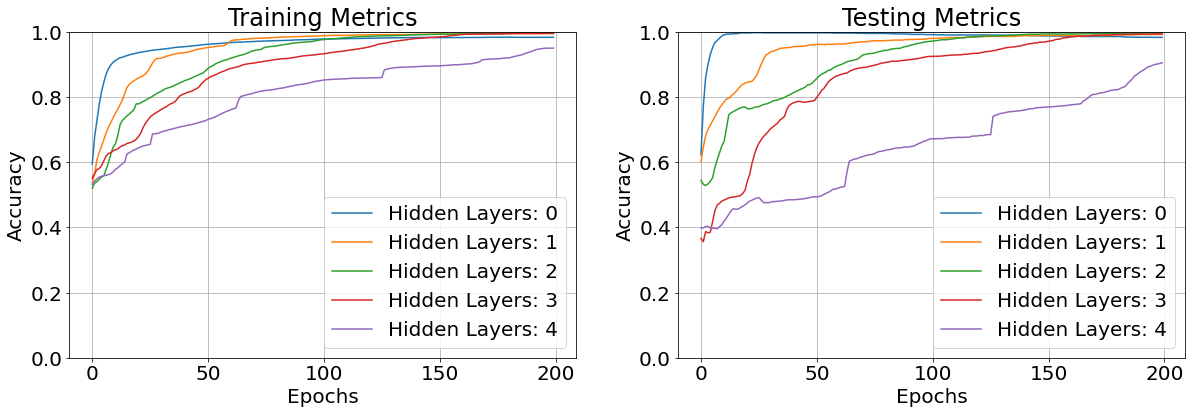
\includegraphics[width=\textwidth]{figs/layers.png}
  \caption{
    Average accuracy across 10 iterations for varied number of hidden
    layers.
  }
  \label{fig:layers}
\end{figure}

\begin{figure}[H]
  \centering
  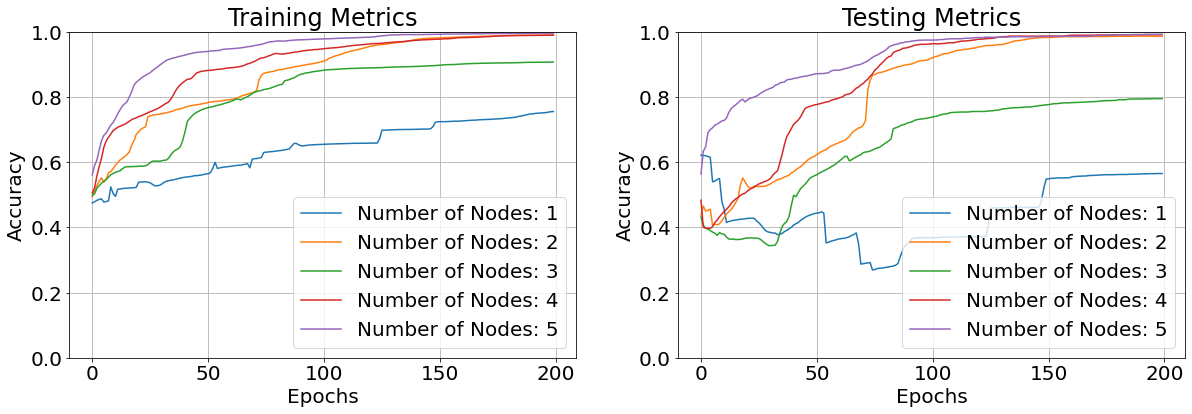
\includegraphics[width=\textwidth]{figs/nodes.png}
  \caption{
    Average accuracy across 10 iterations for varied number of nodes
    in 2 hidden layers.
  }
  \label{fig:nodes}
\end{figure}

\begin{figure}[H]
  \centering
  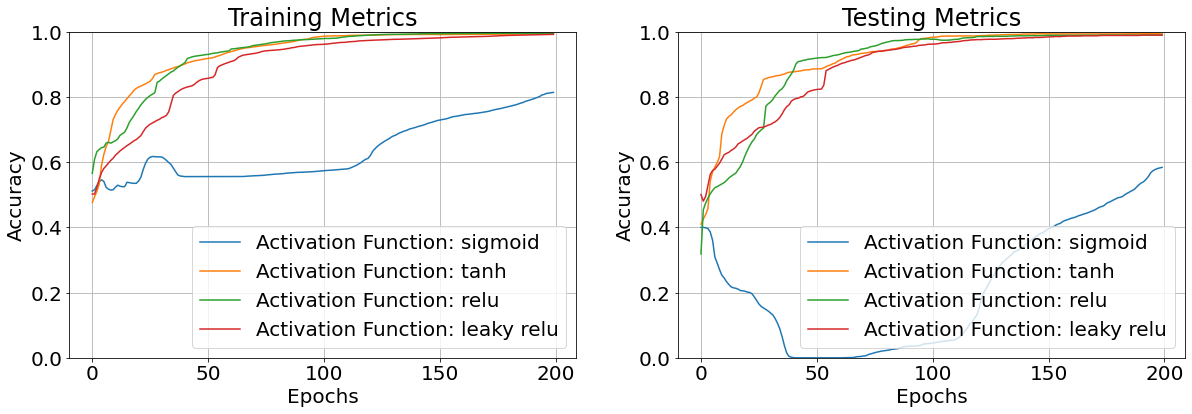
\includegraphics[width=\textwidth]{figs/funcs.png}
  \caption{
    Average accuracy across 10 iterations for differing activation
    functions in 2 hidden layers each with 4 nodes and a learning rate
    \alpha=0.1 .
  }
  \label{fig:funcs}
\end{figure}

\begin{figure}[H]
  \centering
  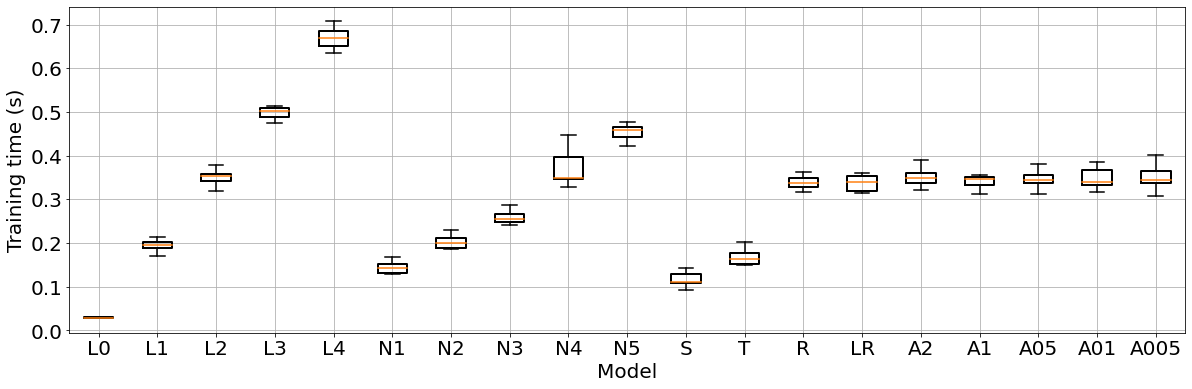
\includegraphics[width=\textwidth]{figs/times.png}
  \caption{
    Average training time of each model across 10 iterations.
    Modified hyperparameter abbraviation identifies each model:
    L = hidden layers, N = nodes, S|T|R|LR = activation function,
    A = learning rate.
  }
  \label{fig:times}
\end{figure}

\section{Discussion and Conclusions}

The number of hidden layers negatively affects a network's learning rate as can be seen in \ref{fig:layers}. Surprisingly, the model with 0 hidden layers (i.e. a perceptron) outperforms the more complex architectures, especially on the test set (\ref{fig:layers}). It seems intuative that initially arbitrary ouputs from preceding layers introduces more epochs to equivalently adjust the weights of following layers. Nonetheless, the model with the single node generalises unexpectedly well to unseen data which is likely a reflection of the simplified dataset used.

Conversely, the number of nodes has a reverse effect on the model's accuracy -- increasing the number of nodes improves the model's performance and ability to generalise to unseen data. Models with fewer nodes are more prone to overfit the data especially in the earlier epochs, characterised by the decreasing accuracy when using testing data (see \ref{fig:nodes}).

The choice of activation function is critical to the model's performance, best demonstrated by the sigmoid model (\ref{fig:funcs}). In the 40 to 120 epoch range singmoid function gets 'stuck' and learning stalls, surprisingly the 40 epoch mark is also when the sigmoid model starts to generalise to the test dataset after severe overfitting up to that point. Nonetheless, by the end of  the 200 epochs, sigmoid model's accuracy is only slightly better than chance, very different from the 0.8 accuracy of the training dataset - a sign of overfitting and overall poor generalisation to unseen data.
Somewhat unexpected is the performance of the Tanh function which is comparable to and even surpasses the ReLU models in terms of accuracy, however this likely reflects the simplicity of this particular clasisfication problem.

A linear relationship between average training time and the number of nodes per hidden layer, as well as the number of hidden layers is observed (\ref{fig:times}). Unexpected is the comparison between training times of models with different activation functions, with Tanh and Sigmoid outperforming the ReLU functions, since ReLU functions forgo the need for expensive exponent computations and divisions, designed to improve computation performance \cite{Niwa}. The results could be explained by the simplified dataset and network architecture used, with the performance benefits of ReLU and its variants becoming evident in more complex networks and classification problems.

Interestingly, training time is unaffected by the model's learning rate. When investigating alpha values further, dips in accuracy are observed, when using very small $\alpha$ values. Perhaps, due to the small gradient, the model gets stuck in a local minima, the minima is likely shallow which larger $\alpha$ values have no trouble escaping, hence the lack of dips in accuracy (see if this changes when the train/test sets are introduced (i.e., training set is reduced) which might have an effect on the landscape of the loss function \cite{Guo}).

Sigmoid and Tanh functions are sensitive to input in their mid-point range (where y = 0.5 and y =0.0 respectively), anything below or above theses values quickly reduces the learning rate (output value close to 0 or 1, any changes to weights have very minor impact) and eventually saturates the gradient.
Tanh output range of -1 to 1 has the advantage of adjusting weights in both positive or negative direction in a single iteration as opposed to sigmoid (justification for improved performance of tanh over sigmoid, reference?).
Rectified learning unit function forgoes learning slowdown encountered by sigmoid and tanh when very large inputs are used (ReLU has no upper limit), however negatively weighted inputs cause neurons to die off, stopping learning altogether. Leaky ReLU (an improved version of ReLU) addresses the issue of dying nodes by assigning negative inputs a small negative value (reference?)..

In retrospect, implementing adaptive learning rate and alternative weight initialisation approaches (e.g. Xavier) could have benefited to a more robust classifier.

\begin{thebibliography}{10}
\bibitem{Nielsen} Michael A. Nielsen, ``Neural Networks and Deep Learning", Determination Press, 2015
\bibitem{Xavier}Xavier Glorot, Yoshua Bengio, ``Proceedings of the Thirteenth International Conference on Artificial Intelligence and Statistics", PMLR 9:249-256, 2010
\bibitem{Guo}  Yangzi Guo, Adrian Barbu, ``A study of local optima for learning feature interactions using neural networks", 2020
\bibitem{Niwa} Chigozie Nwankpa, Winifred Ijomah, Anthony Gachagan, \& Stephen Marshall, ``Activation Functions: Comparison of trends in Practice and Research for Deep Learning'', 2018

\end{thebibliography}

\end{document}